\subsection{Mobile robot}
\label{sec:mobile}

Mobile robots (or telerobot) have the capability to move around
in their environment and are not fixed to one physical location.
\\
As stated in \cite{robot:whereami}, Leonard and Durrant-Whyte
(in 1991) summarized the general problem of mobile robot navigation
by three questions:

\begin{itemize}
\item \texttt{Where am I ?}
\item \texttt{Where am I going ?}
\item \texttt{How should I get there ?}
\end{itemize}

This section surveys the some basic notions in sensors 
and technologies that aim at answering the
first question.
\\
We will often refer to the expression \textit{robot navigation},
that is primarily about guiding a mobile robot to a desired destination
or along a pre-specified path. For these reasons teleoperator must
be able, with an as great as possible precision, to know the robot's
position in its environment, which consists of landmarks and obstacles.
\\
In order to achieve this objective the robot needs to be equipped with
sensors suitable to localise the robot throughout the path it is to follow.
These sensors may give overlapping or complementary information and may
also sometimes be redundant. Because of the lack of a single, generally
good method, developers of  automated guided vehicles (AGVs) and mobile
robots usually combine two or more methods to localize the robot.
\\
All these sensor measurements can be fused to estimate the robot's
position by using a sensor fusion algorithm. Sensor fusion
in this case is the method of integrating data from distinctly
different sensors to estimate the robot's position.
\\
The sensors used to localize the mobile robot can be categorized into
two groups: internal and external sensors. The ones belonging to the first
group measure some internal state of the robot, such as motion, acceleration,
direction.
\\
Sensors belonging to the second group (external sensors) provide information
about objects in the workspace surrounding the robot.
\\
Sensors that will be exposed in this section are:
\begin{itemize}
\item \texttt{Encoder} \\
  Internal sensor, details in chapter \ref{sec:mobile:encoder}
\item \texttt{Laser} \\
  External sensor, details in chapter \ref{sec:mobile:laser}
\item \texttt{Sonar} \\
  External sensor, details in chapter \ref{sec:mobile:sonar}
\item \texttt{Bumper} \\
  External sensor, details in chapter \ref{sec:mobile:bumper}
\item \texttt{Image sensor} \\
  External sensor, details in chapter \ref{sec:mobile:image}
\end{itemize}

Data collected with previous sensors must be processed with proper methods to
determinate robot's position. Among these we will briefly cite: 
\begin{itemize}
\item \texttt{Odometry} \\
  Details in chapter \ref{sec:mobile:odometry}
\item \texttt{Inertial Navigation} \\
  Details in chapter \ref{sec:mobile:inertial}
\item \texttt{Video based positioning} \\
  Details in chapter \ref{sec:mobile:video}
\end{itemize}

%%------------------------------------------------------------------

\subsubsection{Encoder}
\label{sec:mobile:encoder}


The simplest type of incremental encoder is a single-channel
\textit{tachometer encoder}, basically an instrumented mechanical
light chopper that produces a certain number of sine or square wave
pulses for each shaft revolution. Adding pulses increases the resolution
(and subsequently the cost) of the unit.
\begin{figure} [h]
  \begin{center}
    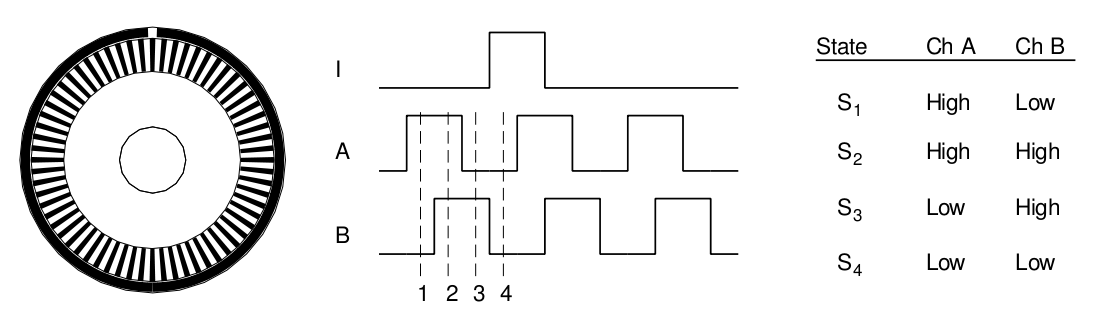
\includegraphics[width=\textwidth]{img/incremental_encoder.png}
    \caption{The observed phase relationship between Channel A and B
      pulse trains can be used to determine
      the direction of rotation with a phase-quadrature encoder,
      while unique output states S1 - S4 allow for up to a
      four-fold increase in resolution. The single slot in the outer
      track generates one index pulse per disk rotation.
    }
    \label{fig:incremental_encoder}
  \end{center}
\end{figure}
These relatively inexpensive devices are well suited as velocity feedback
sensors in medium to high speed control systems, but run into noise and
stability problems at extremely slow velocities due to quantization errors.
\\
The tradeoff here is resolution versus update rate: improved transient
response requires a faster update rate, which for a given line count reduces
the number of possible encoder pulses per sampling interval. 
\\
In addition to low-speed instabilities, single-channel tachometer encoders
are also incapable of detecting the direction of rotation and thus cannot
be used as position sensors. Phase-quadrature incremental encoders overcome
these problems by adding a second channel, displaced from the
first, so the resulting pulse trains are 90 degrees out of phase, as shown
in figure \ref{fig:incremental_encoder}.
\\
This technique allows the decoding electronics to determine which channel
is leading the other and hence ascertain the direction of rotation, with the
added benefit of increased resolution.
\\
The incremental nature of the phase-quadrature output signals dictates that
any resolution of angular position can only be relative to some specific
reference, as opposed to absolute. Establishing such a reference can be
accomplished in a number of ways. For applications involving continuous
360-degree rotation, most encoders incorporate as a third channel a special
index output that goes high once for each complete revolution of the shaft
(see figure \ref{fig:incremental_encoder}).
\\
Intermediate shaft positions are then specified by the number of encoder
up counts or down counts from this known index position.
\\
One disadvantage of this approach is that all relative position information
is lost in the event of a power interruption.
\\
Interfacing an incremental encoder to a computer is not a trivial task.
A simple state-based interface as implied in Figure 1.1 is inaccurate if
the encoder changes direction at certain positions, and false pulses can
result from the interpretation of the sequence of state changes.
\\
Absolute encoders are typically used for slower rotational applications
that require positional information when potential loss of reference
from power interruption cannot be tolerated.
\\
Instead of the serial bit streams of incremental designs, absolute optical
encoders provide a parallel word output with a unique code pattern for each
quantized shaft position. The most common coding schemes are \textit{Gray code},
natural binary, and binary-coded decimal.
\\
The Gray code (for inventor Frank Gray of Bell Labs) is characterised by the
fact that only one bit changes at a time, a decided advantage in eliminating
asynchronous ambiguities caused by electronic and mechanical component tolerances
(see figure \ref{fig:absolute_encoder}a).
\begin{figure} [h]
  \begin{center}
    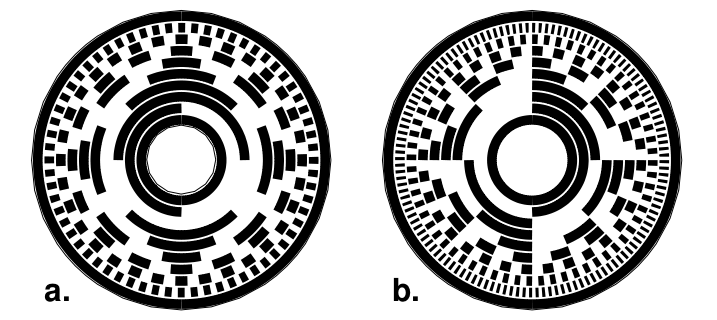
\includegraphics[width=300pt]{img/absolute_encoder.png}
    \caption{Rotating an 8-bit absolute Gray code disk.
      a. Counterclockwise rotation by one position increment will cause
      only one bit to change.
      b. The same rotation of a binary-coded disk will cause all bits to
      change in the particular case (255 to 0) illustrated by the
      reference line at 12 o'clock.}
    \label{fig:absolute_encoder}
  \end{center}
\end{figure}
Binary code, on the other hand, routinely involves multiple bit changes when
incrementing or decrementing the count by one. For example, when going from
position 255 to position 0 in figure \ref{fig:absolute_encoder}b, eight
bits toggle from 1s to 0s. Since
there is no guarantee all threshold detectors monitoring the detector elements
tracking each bit will toggle at the same precise instant, considerable ambiguity
can exist during state transition with a coding scheme of this form.
\\
Some type of handshake line signaling valid data available would be required
if more than one bit were allowed to change between consecutive encoder positions.
\\
Absolute encoders are best suited for slow and/or infrequent rotations such
as steering angle encoding, as opposed to measuring high-speed continuous
(i.e., drive wheel) rotations as would be required for calculating displacement
along the path of travel.
\\
A potential disadvantage of absolute encoders is their parallel data output,
which requires a more complex interface due to the large number of electrical leads.


\subsubsection{Laser}
\label{sec:mobile:laser}

In laser-based systems, also known as \textit{laser radar} or
\textit{lidar}, a beam of light is emitted in a rapid sequence
of short bursts aimed directly at the object being ranged.
\\
The time required for a given pulse to reflect off the object
and return is measured and used to calculate distance to the
target based on the speed of light. Accuracies for early sensors
of this type could approach a few centimeters over the range
of 1 to 5 meters.
\\
The method above is also used in ultrasonic sensors (we refer to
chapter \ref{sec:mobile:sonar} for more details), where sound pulses
are transmitted and the reflection time is measured (also known as
\textit{time of flight} or shortly \textit{TOF}).
\\
The TOF is directly proportional to the distance between the scanner
and the object. By indicating with \textit{L} the distance between
the laser and the obstacle, whereas with \textit{c} the light speed,
the formula to reckon up TOF is:

\[
t_{flight} = \frac{2L}{c}  \Longrightarrow  L = \frac{t_{flight}}{2}\cdot c
\]

The quality of time of flight range sensors manly depends on:

\begin{itemize}
\item Uncertainties about the exact time of arrival of the reflected signal
\item Inaccuracies in the time of fight measure
\item Interaction with the target (surface, specular reflections)
\item Variation of propagation speed
\item Speed of mobile robot and target
\end{itemize}

\begin{figure} [h]
  \begin{center}
    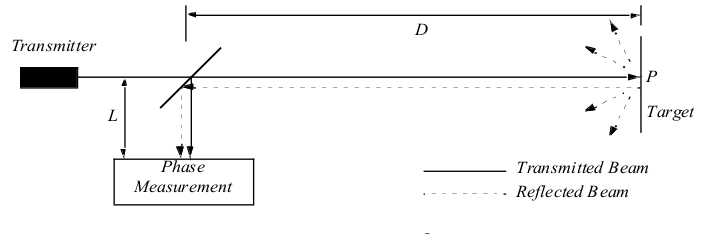
\includegraphics[width=\textwidth]{img/laser_shift_phase.png}
    \caption{Phase-Shift Measurement}
    \label{fig:laser_shift_phase}
  \end{center}
\end{figure}
Another easier method, working with laser beams, is to transmit 100\%
amplitude modulated light beam at a defined frequency and compare
the phase shift between the transmitted and the reflected light (a scheme
is presented in figure \ref{fig:laser_shift_phase}).
\\
This scanner has much higher resolution. The mathematical formulas to
obtain distance follow. We indicate with \textit{f} the modulating
frequency; with \textit{c}, once again, the light speed. We can calculate
the wavelength \textit{$\lambda$} as:

\[
\lambda = \frac{f}{c}
\]

The distance covered by the emitted light, \textit{D'}, referring to
the distances \textit{D} and \textit{L} showed in figure
\ref{fig:laser_shift_phase}, is equal to:

\[
D' = L + 2 \cdot D = L + \frac{\theta}{2\cdot\pi}\cdot\lambda
\]

where \textit{$\theta$} is the phase difference between transmitted
and reflected beacon, return by the module `phase measurement'.
In the end, distance \textit{D} is reckoned by the following formula:

\[
D = \frac{\lambda}{4\cdot\pi}\cdot{\theta}
\]

Confidence in the range (phase estimate) is inversely proportion to
the square of the received signal amplitude.
\begin{figure} [h]
  \begin{center}
    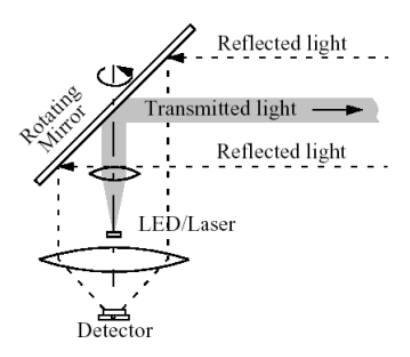
\includegraphics[width=200pt]{img/laser_rotation.png}
    \caption{Schematic drawing of laser range sensor with
      rotation mirror.}
    \label{fig:laser_rotation}
  \end{center}
\end{figure}
Pointing the measuring beam
to rotating mirror a fast scanning can be accomplished in a vertical
dimension, but the whole scanner has to be able to move horizontally
if 3D scanning is needed. A schematic drawing for 2D scanner laser
is showed in figure \ref{fig:laser_rotation}.
\begin{figure} [!h]
  \begin{center}
    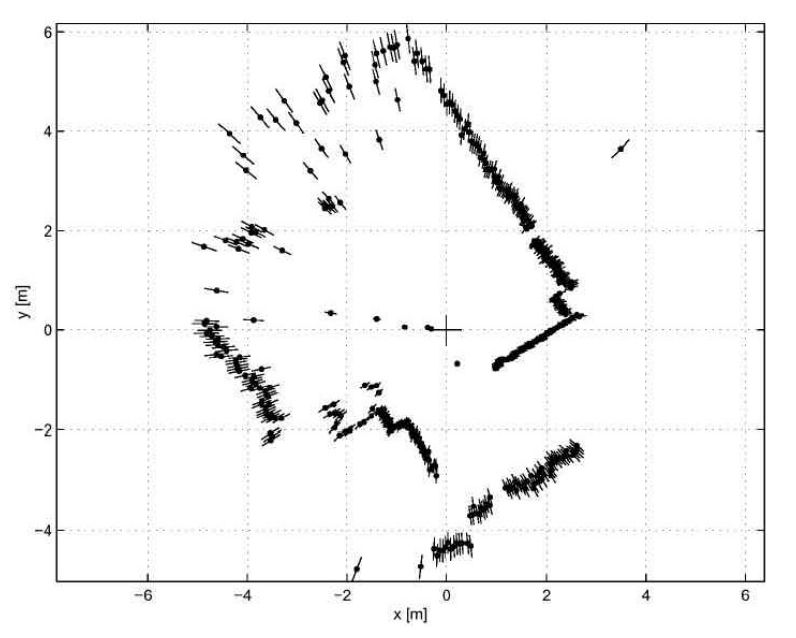
\includegraphics[width=250pt]{img/laser_scan_map.png}
    \caption{Typical range image of a 2D laser range sensor with a
      rotating mirror.}
    \label{fig:laser_scan_map}
  \end{center}
\end{figure}
In figure \ref{fig:laser_scan_map} a typical range image of a 2D
laser range sensor with
a rotating mirror is shown. The lengths of the lines through the
measurement points indicate the uncertainties.


\subsubsection{Sonar}
\label{sec:mobile:sonar}

Ultrasonic TOF ranging is today the most common technique employed
on indoor mobile robotics systems, primarily due to the ready
availability of low-cost systems and their ease of interface.

Active sonar creates an ultrasonic pulse, often called `ping',
then listens for reflections `echo'. Referring to figure
\ref{fig:sonar}, the ping wave is drawn in red, the echo wave
in green.
\begin{figure} [h]
  \begin{center}
    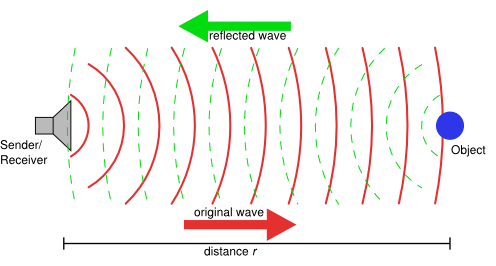
\includegraphics[width=300pt]{img/sonar.png}
    \caption{Sonars in action}
    \label{fig:sonar}
  \end{center}
\end{figure}
\\
The received signal is commonly processed by measuring the time of flight,
already explained in previous section (\ref{sec:mobile:laser}).
This time is depending on the speed of the sound in air, and thus the
temperature, humidity, air pressure, and so on may effect measurements.
\\
The knowledge of time of flight enables the computation of the distance
to the target, which reflected the pulse.
\\
The sonar field of view is a cone and the sensitive area increases
proportionately with the distance. It is necessary to introduce an
inhibition time to avoid the false obstacles due to the ping signal.
On the other hand, the inhibition time does not allow reading
distance too short.
\\
The main drawback with the sonar sensor is its wide beam of perception, which
causes the fact that it is impossible from reading returned data to identify
the object position within the beam. Some of the other sonar drawback are
specular reflection and the possibility of a crosstalk.
\\
Figure \ref{fig:sonar_crosstalk} shows an example of crosstalk.
Crosstalk is a phenomenon in which one sonar picks up the echo
from another. One can distinguish between a. direct effectiveness
of ultrasonic sensors in crosstalk and b. indirect crosstalk.
\begin{figure} [h]
  \begin{center}
    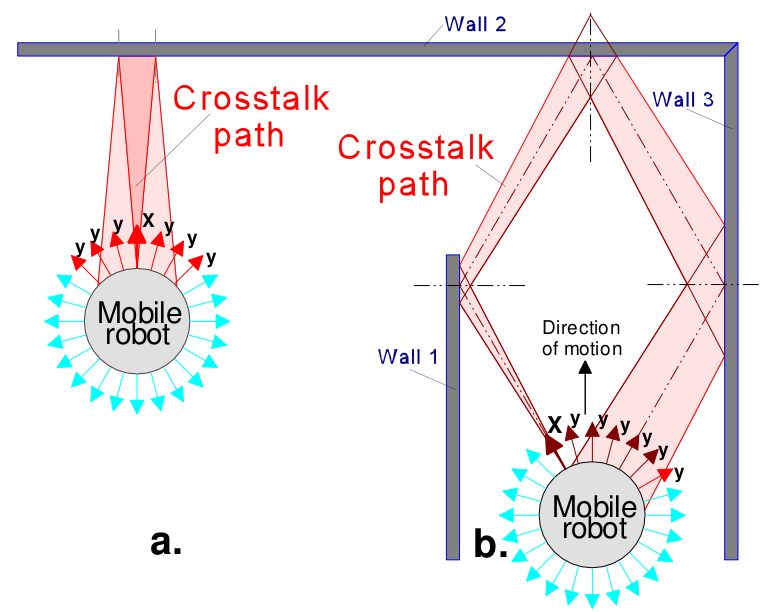
\includegraphics[width=250pt]{img/sonar_crosstalk.png}
    \caption{Example of crosstalk effects with sonar sensors.}
    \label{fig:sonar_crosstalk}
  \end{center}
\end{figure}

\subsubsection{Bumper}
\label{sec:mobile:bumper}

The basic explanation given for why mobile robots need instrumented
bumpers is for a last line of defense type of sensor, one that takes
over if the IR (infra-red), sonar, or other navigational sensors fail
to detect an obstacle. Or, more bluntly, if your other sensors misses
an obstacle, the bumper will indicate the robot has impacted with an
object of unknown size and shape. The robot then can initiate some
sort of evasive/escape maneuvers to
hopefully get back on track to its destination.
\begin{figure} [h]
  \begin{center}
    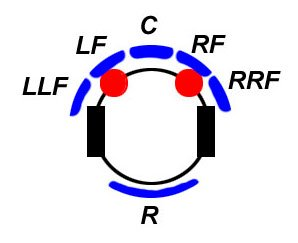
\includegraphics[width=200px]{img/bumpers.jpg}
    \caption{A robot provided with five bumpers, four on front
      side and one on rear side.}
    \label{fig:bumpers}
  \end{center}
\end{figure}
\\
Another advantage of using bumpers is that the impacts derived from
collisions are cushioned, avoiding seriously damages to the robot's
instruments.

\subsubsection{Image sensors}
\label{sec:mobile:image}

An image sensor is a device that converts an optical image to an electric
signal; it is used mostly in digital cameras and other imaging devices.
\\
Early sensors were video camera tubes but a modern one is typically a
charge-coupled device (also known as \textit{CCD}) or a complementary
metal-oxid-semiconductor (\textit{CMOS}) active pixel sensor.
\\
Today, most digital still cameras use either a CCD image sensor or a
CMOS sensor. Both types of sensor accomplish the same task of capturing
light and converting it into electrical signals.
\\
A CCD is an analog device. When light strikes the chip it is held as a small
electrical charge in each photo sensor. The charges are converted to voltage
one pixel at a time as they are read from the chip. Additional circuitry in
the camera converts the voltage into digital information.
\\
A CMOS chip is a type of active pixel sensor made using the CMOS semiconductor
process. Extra circuitry next to each photo sensor converts the light
energy to a voltage; additional circuitry on the chip may be included
to convert the voltage to digital data.
\begin{figure} [h]
  \begin{center}
    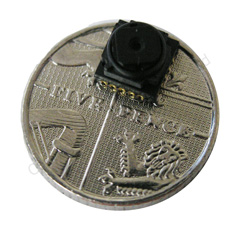
\includegraphics[width=100pt]{img/cmos_camera.jpg}
    \caption{A CMOS camera.}
    \label{fig:cmos_camera}
  \end{center}
\end{figure}
\\
Neither technology has a clear advantage in image quality. On one hand,
CCD sensors are more susceptible to vertical smear from bright light sources
when the sensor is overloaded.
CMOS can potentially be implemented with fewer components, use less power,
and/or provide faster readout than CCDs.
CMOS sensors are less expensive to manufacture than CCD sensors.
\\
There are many parameters that can be used to evaluate the performance
of an image sensor, including its dynamic range, its signal-to-noise ratio,
its low-light sensitivity, etc. For sensors of comparable types,
the signal-to-noise ratio and dynamic range improve as the size increases.
\\
For more details see \cite{wiki:image_sensor}.

\subsubsection{Odometry}
\label{sec:mobile:odometry}

Odometry is the most widely used navigation method for mobile robot
positioning. It is well known that odometry provides good short-term
accuracy, is inexpensive, and allows very high sampling rates. However,
the fundamental idea of odometry is the integration of incremental motion
information over time, which leads inevitably to the accumulation of errors.
\\
Particularly, the accumulation of orientation errors will cause large
position errors which increase proportionally with the distance traveled
by the robot. Despite these limitations, most researchers agree that odometry
is an important part of a robot navigation system and that navigation tasks
will be simplified if odometric accuracy can be improved. Odometry is used
in almost all mobile robots, for various reasons:

\begin{itemize}
\item odometry data can be fused with absolute
  position measurements to provide better and more
  reliable position estimation;
\item odometry can be used in between absolute position updates with
  landmarks. Given a required positioning accuracy, increased accuracy
  in odometry allows for less frequent absolute position updates. As
  a result, fewer landmarks are needed for a given travel distance;
\item many mapping and landmark matching algorithms assume that the robot
  can maintain its position well enough to allow the robot to look for
  landmarks in a limited area;
\item in some cases, odometry is the only navigation information available.
  For example when no external reference is available, when circumstances
  preclude the placing or selection of landmarks in the environment,
  or when another sensor subsystem fails to provide usable data.
\end{itemize}

Odometry is based on simple equations, depending on mobility configuration
chosen for the robot, that are easily implemented and that utilise
data from inexpensive incremental wheel encoders.
\begin{figure} [h]
  \begin{center}
    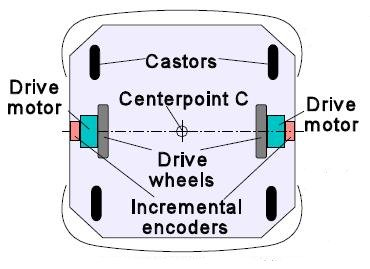
\includegraphics[width=200pt]{img/differential_drive.jpg}
    \caption{A CMOS camera.}
    \label{fig:differential_drive}
  \end{center}
\end{figure}
\\
In \textit{differential-drive}, one of the available robot configuration
shown in figure \ref{fig:differential_drive}, incremental encoders
are mounted onto the two
drive motors to count the wheel revolutions.
\\
The robot can compute, by simple geometric equations, the momentary
position of the vehicle relative to a known starting position.
\\
Suppose that at sampling interval \textit{i} the left and right wheel
encoders show a pulse increment of \textit{$N_{L,i}$} and \textit{$N_{R,i}$},
respectively. Suppose further that

\[
c_m = \frac{\pi \cdot D_n } {n \cdot C_e }
\]

where

\textit{$c_m$} = conversion factor that translates encoder pulses into
linear wheel displacement \\
\textit{$D_n$} = nominal wheel diameter (in mm) \\
\textit{$C_e$} = encoder resolution (in pulses per revolution) \\
\textit{n}   = gear ratio of the reduction gear between the motor
(where the encoder is attached) and the drive wheel \\
\\
we can compute the incremental travel distance for the left and
right wheel, $\bigtriangleup$$U_{L,i}$ and $\bigtriangleup$$U_{R,i}$,
according to

\[
\bigtriangleup U_{L,i} = c_m \cdot N_{L,i}
\]
\[
\bigtriangleup U_{R,i} = c_m \cdot N_{R,i}
\]

and the incremental linear displacement of the robot's centerpoint
\textit{C}, denoted $\bigtriangleup$$U_{i}$, according to

\[
\bigtriangleup U_{i} =
\frac{{\bigtriangleup U_{L,i}} + {\bigtriangleup U_{R,i}}} {2}
\]

Next, we compute the robot's incremental change of orientation

\[
\bigtriangleup \theta_i =
\frac{{\bigtriangleup U_{R,i}} - {\bigtriangleup U_{L,i}}} {b}
\]

where \textit{b} is the wheelbase of the vehicle, ideally measured
as the distance between the two contact points between the wheels
and the floor.
\\
The robot's new relative orientation $\theta_i$ can be computed from
\[
\theta_i = \theta_{i-1} + \bigtriangleup \theta_i
\]

and the relative position of the centerpoint is

\[
x_i = x_{i-1} + \bigtriangleup U_{i} \cdot \cos \theta_i
\]
\[
y_i = y_{i-1} + \bigtriangleup U_{i} \cdot \sin \theta_i
\]

where
\\
\textit{$x_i$}, \textit{$y_i$} = relative position of the
robot's centerpoint \textit{C} at instant i-th.
\\
Unfortunately, odometry is
based on the assumption that wheel revolutions can be translated
into linear displacement relative to the floor.
\\
This assumption is only of limited validity. One extreme example is
wheel slippage: if one wheel was to slip on, say, an oil spill, then
the associated encoder would register wheel revolutions even though
these revolutions would not correspond to a linear displacement of the
wheel.
\\
Along with the extreme case of total slippage, there are several other
more subtle reasons for inaccuracies in the translation of wheel encoder
readings into linear motion. All of these error sources fit into one
of two categories: systematic errors and non-systematic errors.
Systematic errors include:

\begin{itemize}
\item unequal wheel diameters
\item average of actual wheel diameters differs from 
  nominal wheel diameter
\item actual wheelbase differs from nominal wheelbase
\item misalignment of wheels
\item finite encoder resolution
\item finite encoder sampling rate
\end{itemize}

Non-systematic errors include:

\begin{itemize}
\item travel over uneven floors.
\item travel over unexpected objects on the floor.
\item Wheel-slippage due to slippery floors, over-acceleration,
  fast turning (skidding), external or internal forces, non-point wheel
  contact with the floor.
\end{itemize}

The clear distinction between systematic and non-systematic errors is
of great importance for the effective reduction of odometry errors. For example,
systematic errors are particularly grave because they accumulate constantly.
On most smooth indoor surfaces systematic errors contribute much
more to odometry errors than non-systematic errors.
However, on rough surfaces with significant irregularities, non-systematic
errors are dominant.
\begin{figure} [h]
  \begin{center}
    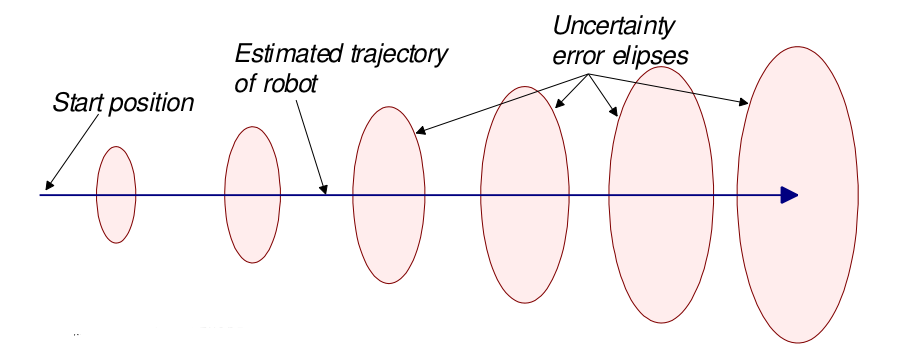
\includegraphics[width=310pt]{img/odometry_error.png}
    \caption{Growing `error ellipses' indicate the growing position
      uncertainty with odometry.}
    \label{fig:odometry_error}
  \end{center}
\end{figure}
\\
The problem with non-systematic errors is that they may appear unexpectedly
(for example, when the robot traverses an unexpected object on the
ground), and they can cause large position errors. Typically, when a mobile
robot system is installed with a hybrid odometry/landmark navigation system,
the frequency of the landmarks is determined
empirically and is based on the worst-case systematic errors. Such systems
are likely to fail when one or more large non-systematic errors occur.
\\
It is noteworthy that many researchers develop algorithms that estimate
the position uncertainty of a robot. With this approach each computed robot
position is surrounded by a characteristic `error ellipse', which
indicates a region of uncertainty for the robot's actual position (see
figure \ref{}).
\\
Typically, these ellipses grow with travel distance, until an absolute
position measurement reduces the growing uncertainty and thereby `resets'
the size of the error ellipse.

\subsubsection{Inertial navigation}
\label{sec:mobile:inertial}

An alternative method for enhancing dead reckoning is
inertial navigation, initially developed for deployment on
aircraft.
\\
The principle of operation involves continuous sensing of minute
accelerations in each of the three directional axes and integrating over time
to derive velocity and position. A gyroscopically stabilized
sensor platform is used to maintain consistent orientation of the three
accelerometers throughout this process.
\\
Although fairly simple in concept, the specifics of implementation are
rather demanding. This is mainly caused by error sources that adversely
affect the stability of the gyros used.
\\
Experimental results indicate that a purely inertial navigation approach
is not realistically advantageous (i.e., too expensive) for mobile robot
applications.
\\
Inertial navigation is attractive mainly because it is self-contained
and no external motion information is needed for positioning. One important
advantage of inertial navigation is its ability to provide fast, low-latency
dynamic measurements.
\\
Furthermore, inertial navigation sensors typically have noise and error sources
that are independent from the external sensors. For example, the noise and error
from an inertial navigation system should be quite different
from that of, say, a landmark-based system.
\\
Fundamentally, gyros provide angular rate and accelerometers provide
velocity rate (i.e. acceleration) information. Dynamic information is
provided through direct
measurements. However, the main disadvantage is that the angular rate data
and the linear velocity rate data must be integrated once and twice (respectively),
to provide orientation and linear position, respectively.
\\
Thus, even very small errors in the rate information can cause an unbounded
growth in the error of integrated measurements.

\subsubsection{Video based positioning}
\label{sec:mobile:video}

A core problem in robotics is the determination of the position and
orientation of a mobile robot in its environment. The basic principles
of landmark-based and map-based positioning also apply to the vision-based
positioning or localization which relies on optical sensors
in contrast to ultrasound, laser and inertial sensors.
Common optical sensors include cameras using CCD arrays.
\\
Visual sensing provides a tremendous amount of information about a
robot's environment, and it is potentially the most powerful source of
information among all the sensors used on robots.
\\
Due to the wealth of information, however, extraction of visual features
for positioning is not an easy task. The problem of localization by vision has
received considerable attention and many techniques have been suggested.
The basic components of the localization process are:

\begin{itemize}
\item representations of the environment
\item sensing models
\item localization algorithms
\end{itemize}

Most localization techniques provide absolute or relative position and/or
the orientation. Techniques vary substantially, depending on the sensors,
their geometric models, and the representation of the environment.
\\
The geometric information about the environment can be given in the form
of landmarks, object models and maps in two or three dimensions. A vision
sensor or multiple vision sensors should capture image features or regions
that match the landmarks or maps.
\\
On the other hand, landmarks, object models, and maps should provide necessary
spatial information that is easy to be sensed. When landmarks or maps of an
environment are not available, landmark selection and map building should
be part of a localization method.
\\
Geometric models of photometric cameras are of critical importance for
finding geometric position and orientation of the sensors. The most common
model for photometric cameras is the pin-hole camera with perspective projection
as shown in figure \ref{fig:camera_system}. Photometric cameras using optical lens can
be modeled as a pin-hole camera.
\begin{figure} [h]
  \begin{center}
    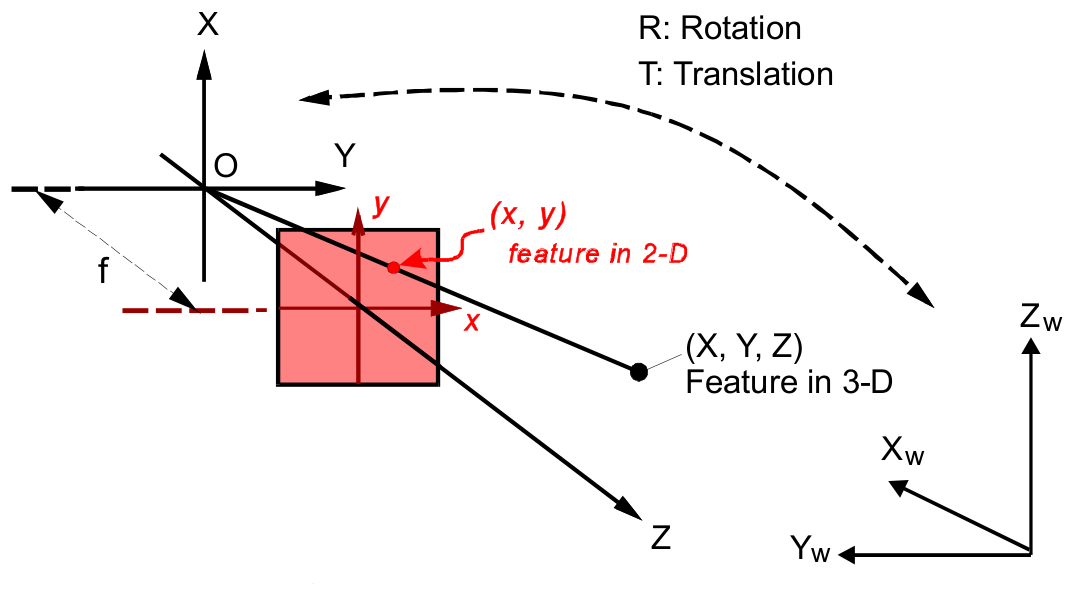
\includegraphics[width=350pt]{img/camera_system.png}
    \caption{Perspective camera model.}
    \label{fig:camera_system}
  \end{center}
\end{figure}
\\
The coordinate system (X, Y, Z) is a three-dimensional camera coordinate
system, and (x, y) is a sensor (image) coordinate system. A three-dimensional
feature in an object is projected onto the image plane (x, y). The relationship
for this perspective projection is given by

\[
x = f \cdot \frac{X}{Z}
\]

\[
y = f \cdot \frac{Y}{Z}
\]

where \textit{f} is the distance the two systems' origins.
\\
Although the range information is collapsed in this projection, the angle or
orientation of the object point can be obtained if the focal length \textit{f}
is known and there is no distortion of rays due to lens distortion.
\\
The internal parameters of the camera are called `intrinsic camera parameters' and
they include the effective focal length f, the radial lens distortion factor,
and the image scanning parameters, which are used for estimating the physical
size of the image plane.
\\
The orientation and position of the camera coordinate system (X, Y, Z) can be
described by six parameters, three for orientation and three for position, and
they are called `extrinsic camera parameters'. They represent the relationship
between the camera coordinates (X, Y, Z) and the world or object coordinates
(XW, YW, ZW).
\\
Landmarks and maps are usually represented in the world coordinate system.
The problem of localization is to determine the position and orientation of a
sensor (or a mobile robot) by matching the sensed visual features in one or
more image(s) to the object features provided by landmarks or maps. Obviously a
single feature would not provide enough information for position
and orientation, so multiple features are required.
\\
Depending on the sensors, the sensing schemes, and the representations of the
environment, localization techniques vary significantly.
